\chapter{Introduction}

\section{Overview}
Java is used in many applications in the industry, and many of those applications use Java Collection Classes. These collection classes contain various Interfaces and their implementations according to the context of different data structures. Java Collection classes provides access to all these data structures so that there is no need to implement them again and again by the user. The performance of these classes has got a huge impact on the performance of many applications in real life. The goal of this project is to improve the perfomance of applications that use Collection class methods with our proposed Collection Class Access oPtimization (CCAP) tool.

\section{Example}
Figure 1.1 program tries to extract the k smallest elements from an ArrayList by sorting the array and iterating over the array for k times.
\begin{lstlisting}[style=java]
// Example.java
import java.util.*;
public class Example {
    public static void main(String[] args) {
        List<Integer>l1 = new ArrayList<>();

        l1.add(10);
        l1.add(4);
        l1.add(5);
        l1.add(15);
        l1.add(20);
        l1.add(14);
        l1.add(35);
        l1.add(17);
        l1.add(19);
        l1.add(40);
        l1.add(21);
        l1.add(3);
        l1.add(27);
        Collections.sort(l1);
        int k = 4;
        for(int i=0;i<k;i++)
            System.out.println(l1.get(i));
    }
}

\end{lstlisting}
\begin{figure} [h]
    \centering
    %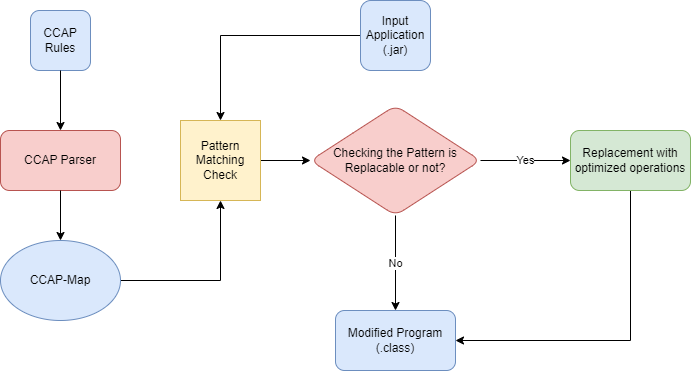
\includegraphics[width = \textwidth]{images/CCAP_tool.png}
    \caption{Sample Java program}
    \label{fig:my_label}
\end{figure}
Here instead of sorting the whole array list and then iterating over the first k elements, (which will take O(nlogn+k) time, where n is the size of the list) we could make a priority queue in O(n) time and extract each min element from the list in O(log n) time. It will reduce the time complexity by a significant amount for large inputs.
\begin{lstlisting}[style=java]
        PriorityQueue pq = new PriorityQueue<>(l1);
        int k = 4;
        for(int i=0;i<k;i++)
        System.out.println(pq.poll());

\end{lstlisting}
\begin{figure} [h]
    \centering
    %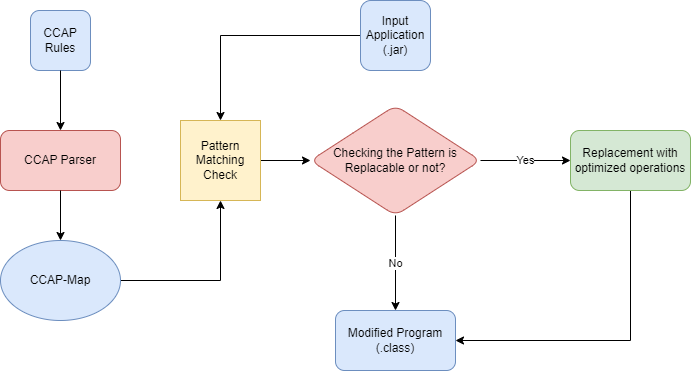
\includegraphics[width = \textwidth]{images/CCAP_tool.png}
    \caption{The proposed replacement code for the last 4 lines of Fig1.1}
    \label{fig:my_label}
\end{figure}

As shown above the time complexity for making a priority queue is in O(n) and for polling, it will take O(log n) so overall it will be O(n+klogn) only. So for smaller k values and larger n Values, it will make a very big change in time complexity. For larger values of k, the cost of the proposed modified code is comparable to the original code.

We call functions like Sort, that iterate over nearly all the elements of the collection as "Expensive functions" and functions that iterate over very small number of elements in the resulting collections as "Cheaper functions". Our goal is to replace calls to expensive functions with other alternatives so that the following calls to the cheaper functions can be realized without paying the high cost of expensive functions.
Telkunte \cite{MTP_2017} had identified that different generic Java library methods can be optimized based on this specific uses. Kiran \cite{Vishnu_Kiran} had written a preliminary tool to identify such segment of methods. In this work we provide a mechanism to identify sequence of optimizable patterns and a tool to automatically optimize applications that have such patterns.

\section{Major Contributions}
\begin{enumerate} [blt]
    \item fixed the "Follow-up" \cite{Vishnu_Kiran} tool to identify the patterns of access by Java Collection class functions. 
    \item a grammar (CCAP grammar) is created for rules using which we can specify which type of patterns to replace.
    \item we have created a list of patterns which can be optimized.
    \item A parser is developed with which we can read the rules from user and generates a CCAP-map which contains the mappings of original patterns with optimized versions.
    \item An Algorithm was designed and developed that is able to replace the patterns with optimized versions in input Java applications.
    \item Created a set of micro benchmarks which contains the code with these patterns and then tested the CCAP tool on these microbenchmarks with high degree of success. 
\end{enumerate}
